% The Slide Definitions
%document
\documentclass[10pt]{beamer}
%theme
% \usetheme{metropolis}
% packages
\usepackage{color}
\usepackage{listings}
\usepackage[ngerman]{babel}
\usepackage[utf8]{inputenc}
\usepackage{multicol}


% color definitions
\definecolor{mygreen}{rgb}{0,0.6,0}
\definecolor{mygray}{rgb}{0.5,0.5,0.5}
\definecolor{mymauve}{rgb}{0.58,0,0.82}

\lstset{
    backgroundcolor=\color{white},
    % choose the background color;
    % you must add \usepackage{color} or \usepackage{xcolor}
    basicstyle=\footnotesize\ttfamily,
    % the size of the fonts that are used for the code
    breakatwhitespace=false,
    % sets if automatic breaks should only happen at whitespace
    breaklines=true,                 % sets automatic line breaking
    captionpos=b,                    % sets the caption-position to bottom
    commentstyle=\color{mygreen},    % comment style
    % deletekeywords={...},
    % if you want to delete keywords from the given language
    extendedchars=true,
    % lets you use non-ASCII characters;
    % for 8-bits encodings only, does not work with UTF-8
    frame=single,                    % adds a frame around the code
    keepspaces=true,
    % keeps spaces in text,
    % useful for keeping indentation of code
    % (possibly needs columns=flexible)
    keywordstyle=\color{blue},       % keyword style
    % morekeywords={*,...},
    % if you want to add more keywords to the set
    numbers=left,
    % where to put the line-numbers; possible values are (none, left, right)
    numbersep=5pt,
    % how far the line-numbers are from the code
    numberstyle=\tiny\color{mygray},
    % the style that is used for the line-numbers
    rulecolor=\color{black},
    % if not set, the frame-color may be changed on line-breaks
    % within not-black text (e.g. comments (green here))
    stepnumber=1,
    % the step between two line-numbers.
    % If it's 1, each line will be numbered
    stringstyle=\color{mymauve},     % string literal style
    tabsize=4,                       % sets default tabsize to 4 spaces
    % show the filename of files included with \lstinputlisting;
    % also try caption instead of title
    language = Python,
	showspaces = false,
	showtabs = false,
	showstringspaces = false,
	escapechar = ,
}

\def\ContinueLineNumber{\lstset{firstnumber=last}}
\def\StartLineAt#1{\lstset{firstnumber=#1}}
\let\numberLineAt\StartLineAt



\newcommand{\codeline}[1]{
	\alert{\texttt{#1}}
}

\def\codewithsource#1{
    \lstinputlisting{#1}
    \textcolor{blue}{\url{#1}}
}


% Author and Course information
% This Document contains the information about this course.

% Authors of the slides
\author{Felix Döring, Felix Wittwer, Anton Obersteiner}

% Name of the Course
\institute{Python-Kurs}

% Fancy Logo 
\titlegraphic{\hfill
\includegraphics[height=1.25cm]{../templates/fsr_logo_cropped}}



% Custom Bindings
% \newcommand{\codeline}[1]{
%	\alert{\texttt{#1}}
%}


% Presentation title
\title{Git}
\author{Anton Obersteiner}
\date{\today}

\usepackage{tikz}
\usepackage{chemarrow}
\def\Ra[#1]#2{++(0, .2) arc [start angle=110, end angle= 70, radius=#1] node[near start, above] {#2}}
\def\Rb[#1]#2{++(0,-.2) arc [start angle=-70, end angle=-110, radius=#1] node[near start, below] {#2}}
\newcommand\pic{\begin{tikzpicture}
	\node (working) at (0, 0) {working};
	\node (stage) at (2, 0) {stage};
	\node (repo) at (4, 0) {repo};
	\node (remote) at (6, 0) {remote};

	\draw[-latex] (working) -- node[above] {\tt add} (stage);
	\draw[-latex] (stage) \Ra[3cm]{\tt commit} (repo);
	\draw[-latex] (repo) \Rb[6cm]{\tt checkout} (working);
	\draw[-latex] (repo) \Ra[3cm]{\tt push} (remote);
	\draw[-latex] (remote) \Rb[3cm]{\tt pull} (repo);
\end{tikzpicture}}

\begin{document}

\maketitle

\begin{frame}{Gliederung}
	\setbeamertemplate{section in toc}[sections numbered]
	\tableofcontents
\end{frame}

\section{Wozu?}
\begin{frame}{Wozu?}
	\begin{itemize}
		\item Versionen und Änderungen speichern
		\item alte Zustände wiederherstellen
		\item Verschiedene Änderungen vergleichen
		\item und zusammenführen
	\end{itemize}
\end{frame}

\subsection{Beispiele}
\begin{frame}{Dateien/Änderungen verschieben}
	\begin{description}
		\item[Code]<1-> Module getrennt entwickeln
		\item[Features]<2-> entwickeln, ohne Funktionierendes zu gefärden
		\item[Bugs]<3-> Finden: durch Vergleich von älteren Zuständen
		\item[Texte]<4-> Dokumentation \& sonstige gemeinsame Texte
		\item[Recht]<5-> Gesetzesänderungen transparent darstellen
	\end{description}
	\begin{figure}
		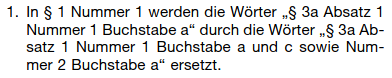
\includegraphics[width=.5\linewidth]{verordnung.png}
		\caption{Erste Verordnung zur Änderung der Mobilitätsdatenverordnung
		Vom 6. Januar 2022}
		\label{fig:verordnung}
	\end{figure}
\end{frame}

\section{Dateien/Änderungen verschieben}
\section{Befehle: {\tt git <...>}}
\subsection{Ebenen}
\begin{frame}{Befehle: {\tt git <...>}: Ebenen}
	\begin{description}
		\item[working]<1->	Inhalt des Ordners
		\item[stage]<2->	``Auf dem Tisch'', Fertig für Commit
		\item[commit]<3->	Paket von Änderungen (klein, ``nur eine Sache'')
		\item[branch]<4->	Reihe zusammenhängender Commits (ein größeres Thema)
		\item[repo]<5->		Gesamt-Sammlung der Commits
		\item[remote]<6->	Online-Repo (Von gesamter Gruppe, ...)
		\item[commit]<7->	aktuelle Stage zusammenfassen und abspeichern
	\end{description}
	\begin{tikzpicture}
		\node (working) at (0, 0) {working};
		\onslide<2->{\node (stage) at (2, 0) {stage};}
		\onslide<5->{\node (repo) at (4, 0) {repo};}
		\onslide<6->{\node (remote) at (6, 0) {remote};}

		\onslide<2->{\draw[-latex] (working) -- node[above] {\tt add} (stage);}
		\onslide<3->{\draw[-latex] (stage) \Ra[3cm]{\tt commit} (repo);}
		\onslide<8->{\draw[-latex] (repo) \Rb[6cm]{\tt checkout} (working);}
		\onslide<6->{\draw[-latex] (repo) \Ra[3cm]{\tt push} (remote);}
		\onslide<7->{\draw[-latex] (remote) \Rb[3cm]{\tt pull} (repo);}
	\end{tikzpicture}
\end{frame}

\subsection{Basic}
\begin{frame}{Befehle: {\tt git <...>}: Basic}
	\begin{description}
		\item[init]<1->		neues GitRepo anlegen
		\item[status]<2->	Was ist neu in Working und Stage
		\item[log]<3-> 		vergangene Commits/Änderungen
		\item[add]<4-> 		Dateien/Änderungen hinzufügen (zu Stage)
		\item[commit]<5->	aktuelle Stage zusammenfassen und abspeichern
	\end{description}
	\pic
\end{frame}

\subsection{Management}
\begin{frame}{Befehle: {\tt git <...>}: Management}
	\begin{description}
		\item[diff]<1->		Unterschiede zwischen Repo und Working
		\item[rm]<2->		Datei löschen (muss man committen)
		\item[mv]<3->		Datei umbenennen (muss man committen)
		\item[checkout]<4->	Commit/Dateien aus Repo in Working laden
		\item[reset HEAD]<5->	aus Stage in Working schieben
		\item[branch]<6->	Ideen ausprobieren $\to$ nicht den Hauptzweig zuschreiben
		\item[merge]<7->	Änderungen in aktuellen Branch übernehmen
	\end{description}
	\pic
\end{frame}

\subsection{Online/Remote}
\begin{frame}{Befehle: {\tt git <...>}: Online/Remote}
	\begin{description}
		\item[remote]<1->	Online-repository anbinden
		\item[clone]<2->	remote lokal kopieren (in Ordner ohne Git)
		\item[fetch]<3->	remote anfragen
		\item[pull]<4->		remote in lokal mergen
		\item[push]<5->		lokal in remote mergen
		\item[fork]<6->		eigene Kopie von fremdem Repo erstellen
		\item[pull request]<7->	fremdem Repo Änderung vorschlagen
	\end{description}
	\pic
\end{frame}

\subsection{Kultur am Ende}
\begin{frame}{Kultur am Ende}
	\begin{description}
		\item[commit]<1-> Macht eine Sache (Plugin oder {\tt git add -p})
		\item[commit]<2-> Kurze, aber präzise Beschreibung
		\item[main]<3-> Stabiler Branch, in den man nur Fertiges mergt
		\item[develop]<4-> Für aktuellen gemeinsamen Stand
		\item[user/topic]<5-> Mögliches Benennungsschema
		\item[remerge]<6-> vermeiden, develop oder master in topic zu mergen
	\end{description}
\end{frame}

% nothing to do from here on
\end{document}
